\chapter{SAC Headers}\label{cha:SAC-headers}

Information about the simulation (i.e., event/station information, sampling rate, etc.)
is written in the header of the seismograms in SAC format.
The list of values and related explanation are given in Figure \ref{fig:SAC-headers}.
Please check the \href{http://www.iris.edu/software/sac/}{SAC webpages} for further information.
Please note that the reference time KZTIME is the centroid time ($t_\text{CMT}=t_\text{PDE}+\texttt{time shift}$)
which corresponds to zero time in the synthetics.
For kinematic rupture simulations, KZTIME is equal to the CMT time of the source having the minimum time-shift
in the \texttt{CMTSOLUTION} file, and coordinates, depth and half-duration of the event are not provided in the headers.
%
\begin{figure}[htp]
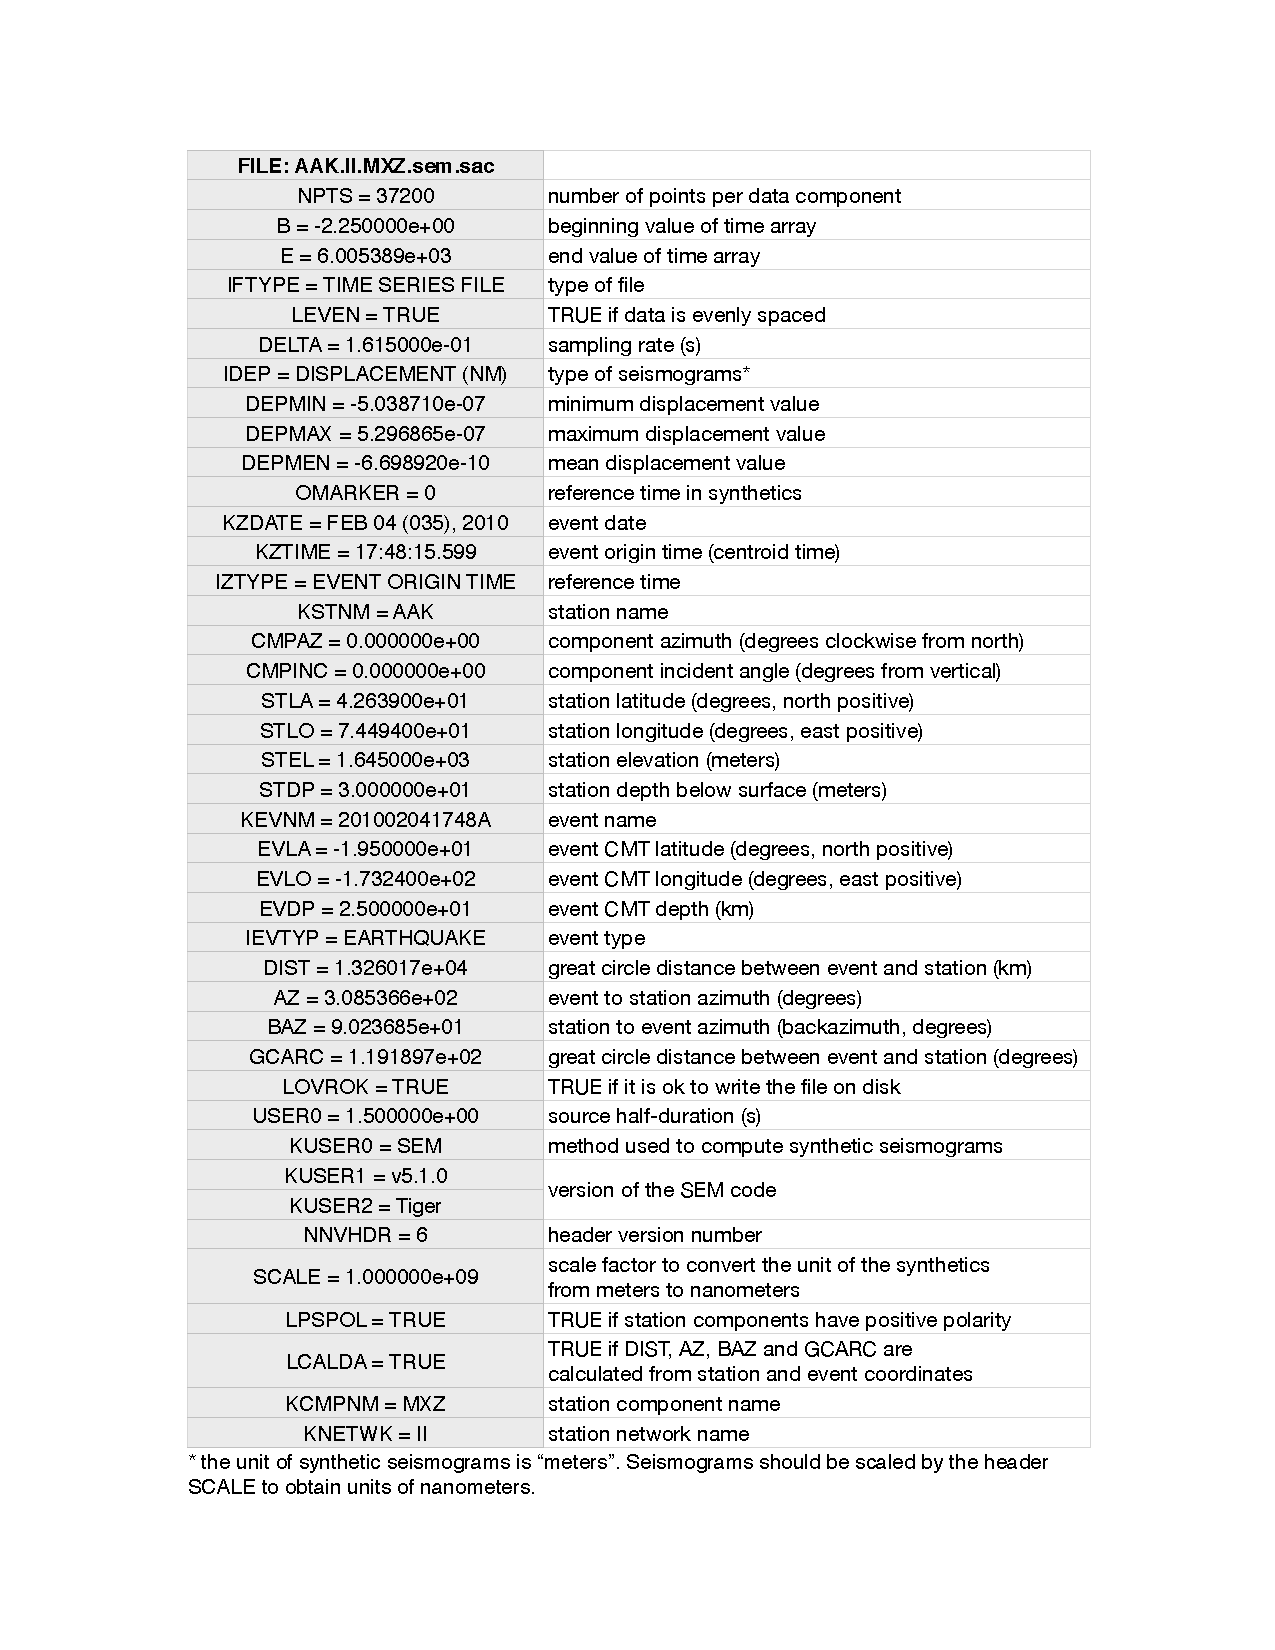
\includegraphics[scale=0.85]{figures/headers_sem_explained.pdf}
\caption{List of SAC headers and their explanations for a sample seismogram.}
\label{fig:SAC-headers}
\end{figure}




